\documentclass{vilniustech}
\vilniustechsetup{
    university={Vilniaus Gedimino technikos universitetas},
    faculty={Fundamentinių mokslų fakultetas},
    cathedral={Matematinės statistikos katedra},
    workTitle={Mokslinių tyrimų ir inovacijų pagrindų},
    workType={Namų darbas nr.1},
    workAuthorGroup={ITSfm-22},
    workAuthorName={Aurimas Šakalys},
    workRecipient={doc. dr. Rūta Simanavičienė}
}
\addbibresource{hw1.bib}
\VTDocumentBegin

\section{System security assurance: A systematic literature review}

\subsection{Straipsnio bibliografinis aprašas}
\VTTable{[
    caption = {Straipsnio bibliografinis aprašas},
    label = {biblio1:short}
    ]{
    colspec = {X[2] X[5]},
    column{1} = {font=\bfseries}
    }
    Autorius (-iai) & Ankur Shukla, Basel Katt, Livinus Obiora Nweke, Prosper Kandabongee Yeng, Goitom Kahsay Weldehawaryat \\
    Pavadinimas & System security assurance: A systematic literature review \\
    Publikavimo metai & 2022 \\
    Žurnalo pavadinimas, vol. & Computer Science Review, 45 \\
    Nuoroda į šaltinį & \url{https://doi.org/10.1016/j.cosrev.2022.100496} \\
}

\subsection{Kokia mokslinė problema sprendžiama analizuojamame darbe?}
Straipsnyje \parencite{SHUKLA2022100496} analizuojama sistemų saugos užtikrinimo metodika. Į analizę įtraukiami dėl informacijos ir komunikacijų technologijų (ICT) atsiradę įšukiai, kadangi įprastai naudojami sprendimai gali neapimti naujai kylančių problemų. Bendrieji kriterijai (CC) naudojami vertinant sistemų saugą yra riboti ir nepaslankūs.

\subsection{Darbo tikslas, keliamas analizuojamame darbe}
Atlikti sistemingą egzistuojančių reikalavimų, procesų ir veiklų analizę sistemų saugos užtikrinimui ir įvardinti esamus trūkumus.

\subsection{Uždaviniai, formuluojami analizuojamame darbe}
Kadangi straipsnyje \parencite{SHUKLA2022100496} atliekama sisteminė analizė, uždaviniai formuluojami tyrimo klausimais.

\VTTable{[
    caption = {Straipsnio keliami klausimai},
    label = {tasks1:short}
    ]{
    colspec = {X[1] X[18]},
    row{1} = {font=\bfseries}
    }
    Nr. & Klausimas \\
    1 & Kokios yra dabartinės tendencijos, sistemų saugos užtikrinimo srityje, apžvelgiant į procesus, metodus, gaires, įrankius,
    metrikas, įvertinimus/technikas, automatizavimą, standartus, ir
    taikomųjų programų dalykines sritis?\\
    2 & Su kokiais iššūkiais, apribojimais ir spragomis susiduriama sistemų saugos užtikrinimo srityje?\\
    3 & Kokios ateities tendencijos sistemų saugos užtikrinimo srityje? \\
    4 & Kaip galėtume klasivikuoti tiriamąją veiklą sistemų saugos užtikrinimo srityje?  \\
}

\subsection{Koks yra mokslinio darbo naujumas?}

\subsection{Koks literatūros apžvalgos tipas taikomas?}

\subsection{Koks empirinio tyrimo metodas taikomas?}

\subsection{Kokie statistiniai metodai taikomi duomenų analizei?}

\subsection{Kurį Bloom'o taksonomijos lygmenį atitinka šis mokslinis darbas ir kodėl?}

\subsection{Koks citavimo stilius naudojamas šiame darbe?}
Cituojama IEEE citavimo stiliumi.

\subsection{Kokioms mokslinių publikacijų citavimo duomenų bazėms priklauso žurnalas, kuriame publikuojamas šis straipsnis?}
\VTTable{[
    caption = {Straipsnio mokslometriniai rodikliai ir duomenų bazės},
    label = {scimetrics1:short}
    ]{
    colspec = {X[5] X[2] X[2]},
    row{1} = {font=\bfseries}
    }
    Duomenų bazės & CiteScore & Impact Factor \\
    ???? & 14.3 & 8.757 \\
}

\section{Standardizing information security - a structurational analysis}

\subsection{Straipsnio bibliografinis aprašas}
\VTTable{[
    caption = {Straipsnio bibliografinis aprašas},
    label = {biblio2:short}
    ]{
    colspec = {X[2] X[5]},
    column{1} = {font=\bfseries}
    }
    Autorius (-iai) & Annika Andersson, Karin Hedström, Fredrik Karlsson \\
    Pavadinimas & Standardizing information security - a structurational analysis \\
    Publikavimo metai & 2022 \\
    Žurnalo pavadinimas, vol., iss. & Information \& Management, 59, 3 \\
    Nuoroda į šaltinį & \url{https://doi.org/10.1016/j.ins.2022.07.053} \\
}

\subsection{Kokia mokslinė problema sprendžiama analizuojamame darbe?}
\subsection{Darbo tikslas, keliamas analizuojamame darbe}
\subsection{Uždaviniai, formuluojami analizuojamame darbe}
\subsection{Koks yra mokslinio darbo naujumas?}
\subsection{Koks literatūros apžvalgos tipas taikomas?}
\subsection{Koks empirinio tyrimo metodas taikomas?}
\subsection{Kokie statistiniai metodai taikomi duomenų analizei?}
\subsection{Kurį Bloom'o taksonomijos lygmenį atitinka šis mokslinis darbas ir kodėl?}

\subsection{Koks citavimo stilius naudojamas šiame darbe?}
Cituojama IEEE citavimo stiliumi.

\subsection{Kokioms mokslinių publikacijų citavimo duomenų bazėms priklauso žurnalas, kuriame publikuojamas šis straipsnis?}
\VTTable{[
    caption = {Straipsnio mokslometriniai rodikliai ir duomenų bazės},
    label = {scimetrics2:short}
    ]{
    colspec = {X[5] X[2] X[2]},
    row{1} = {font=\bfseries}
    }
    Duomenų bazės & CiteScore & Impact Factor \\
    ???? & 13.1 & 10.328 \\
}

\section{Literatūra}

\section{Citavimo pavyzdžiai}

\subsection{Įvairių objektų citavimas}

Tinklalapio citavimas \parencite{webcitation}.
\begin{verbatim}
    \parencite{webcitation}
\end{verbatim}

Straipsnio citavimas \parencite{articlecitation}.
\begin{verbatim}
    \parencite{articlecitation}
\end{verbatim}

Knygos citavimas \parencite{bookcitation}.
\begin{verbatim}
    \parencite{bookcitation}
\end{verbatim}


\subsection{Citavimo komandos}

Parastas citavimas \cite{articlecitation}.
\begin{verbatim}
    \cite{articlecitation}
\end{verbatim}

Citavimas skliausteliuose \parencite{articlecitation}.
\begin{verbatim}
    \parencite{articlecitation}
\end{verbatim}

Citavimas poraštėje \footcite{articlecitation}.
\begin{verbatim}
    \footcite{articlecitation}
\end{verbatim}

Citavimas tekstu \textcite{articlecitation}.
\begin{verbatim}
    \textcite{articlecitation}
\end{verbatim}

\newpage
\section{Iliustracijų/lentelių pavyzdžiai}

\begin{figure}[H]
\begin{center}
    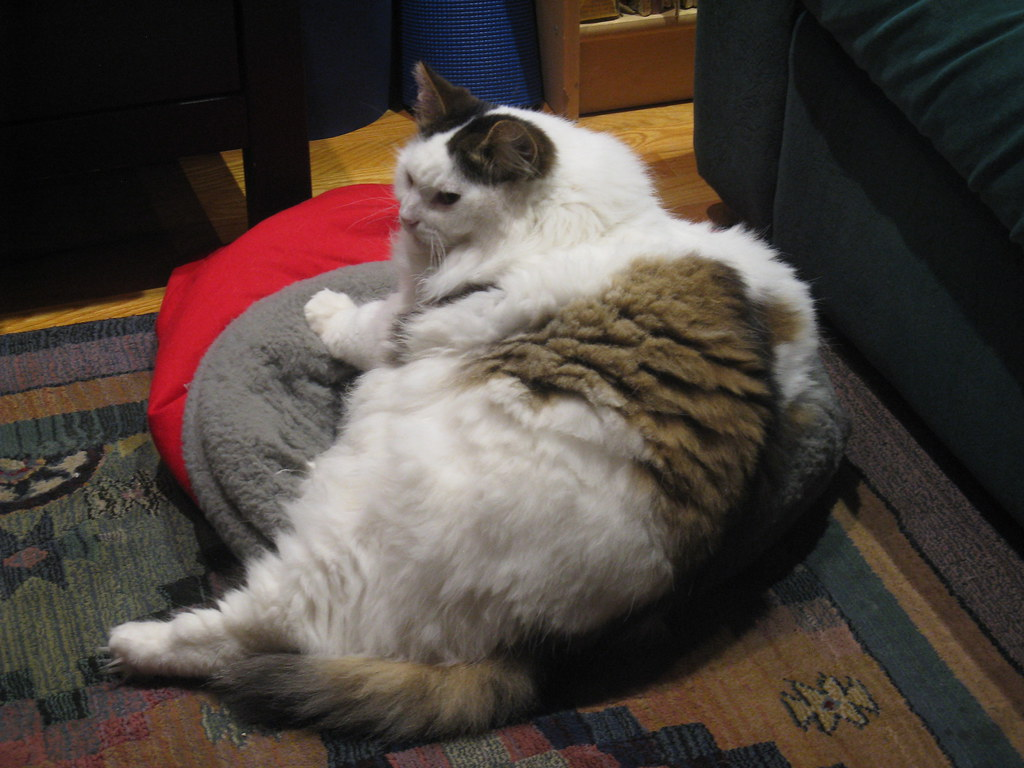
\includegraphics[height=6cm]{img/chonker.jpg}
    \caption{Gabalainis}
    \label{fig:fig1}
\end{center}
\end{figure}

\VTTable{[
    caption = {Trumpa lentelė},
    label = {table:short}
    ]{
    colspec = {XX},
    row{1} = {font=\bfseries}
    }
    Antraštė 1 & Antraštė 2 \\
    Lorem ipsum & Lorem ipsum \\
    Lorem ipsum & Lorem ipsum \\
}

\subsection{Nuorodos}

Nuoroda į iliustraciją \ref{fig:fig1} esančią \pageref{fig:fig1} puslapyje.
\begin{verbatim}
    \ref{fig:fig1} \pageref{fig:fig1}
\end{verbatim}

Nuoroda į trumpą lentelę \ref{table:short} esančią \pageref{table:short} puslapyje.
\begin{verbatim}
    \ref{table:short} \pageref{table:short}
\end{verbatim}

Nuoroda į ilgą lentelę \ref{table:long} esančią \pageref{table:long} puslapyje.
\begin{verbatim}
    \ref{table:long} \pageref{table:long}
\end{verbatim}

\VTTable{[
    caption = {Kelių puslapių lentelė},
    label = {table:long}
    ]{
    colspec = {XXX},
    rowhead = 1,
    row{1} = {font=\bfseries}
    }
    Antraštė 1 & Antraštė 2 & Antraštė 3 \\
    Lorem ipsum & Lorem ipsum & Lorem ipsum \\
    Lorem ipsum & Lorem ipsum & Lorem ipsum \\
    Lorem ipsum & Lorem ipsum & Lorem ipsum \\
    Lorem ipsum & Lorem ipsum & Lorem ipsum \\
    Lorem ipsum & Lorem ipsum & Lorem ipsum \\
    Lorem ipsum & Lorem ipsum & Lorem ipsum \\
    Lorem ipsum & Lorem ipsum & Lorem ipsum \\
    Lorem ipsum & Lorem ipsum & Lorem ipsum \\
    Lorem ipsum & Lorem ipsum & Lorem ipsum \\
}

\VTDocumentEnd